\chapter{Requirements: methodology and use cases}
\label{chap:requisiti}

\section{Requirements methodology}

The requirements of RAM-USB are collected in a single document called the Software Requirements
Specification (SRS) \cite{ramusb-srs},
which constitutes the single source of truth about what the system must do.
The writing of this document follows a spiral model of software engineering \cite{Boehm88},
driven by the progressive resolution of risk, understood as the most significant sources of uncertainty
in the project.
The level of detail of the SRS consequently increases at every iteration because, although
the objectives and the high-level requirements were clear from the initial phases, the knowledge of the
third-party tools and technologies was not sufficient to predict with certainty the low-level behavior
of these tools. The choice of the spiral model stems from this imbalance.
Indeed, many concrete constraints emerged only at implementation time, when direct
interaction with these tools revealed details that a purely theoretical analysis phase was not
able to anticipate.
A concrete case of this dynamic is requirement \texttt{NM-F-12}, revisited in three successive rounds:

in version 1.0 of the SRS \cite{ramusb-commit-nm-f-12-v1} the requirement assumed that Network-Manager (the
component responsible for the private network of the system) had to build from scratch its own mechanism
for authorizing the access of new devices;

in version 1.4 \cite{ramusb-commit-nm-f-12-cli} it emerged that Headscale, the network coordination
tool employed by the system, already offered this functionality through its own
CLI, eliminating the need to write it;

in version 1.7 \cite{ramusb-commit-nm-f-12-14-rework} a deeper limitation of Headscale itself emerged
(it cannot coordinate a network it is part of), examined in depth in
\autoref{sec:paradosso-coordinatore}, requiring a broader reformulation of the requirement.

\section{Requirements traceability}

A distinctive methodological aspect of the project is traceability, understood as a technical constraint
verifiable in three independent directions.
This approach favors ease of security auditing at the cost of a more complex implementation
workflow.

\begin{itemize}
    \item \textbf{From the requirement to its implementation}: every requirement of the SRS that already has an implementation is linked
    to a GitHub permalink pointing to a specific commit and to a precise range of lines.

    \item \textbf{From the test to the requirement and vice versa}: every test function carries, as a documentation comment
    on the line immediately preceding it, the identifier of the requirement it verifies.
    The relation is not necessarily one-to-one, since a requirement can have multiple tests that verify it.
    Moreover, traceability holds in both directions: one can go from the requirement
    to the tests, by searching for the ID in the codebase; and from the test to the requirement, by reading the comment above the function.
    \item \textbf{From the commit to the requirement}: every commit in the repository follows a fixed grammar,
    described in
    \texttt{CONTRIBUTING.md} \cite{ramusb-contributing-commit-structure}
     and summarized here as type, area, description of the change,
    followed by the list of identifiers of the requirements it covers.
    As with the test-requirement link, this too holds in both directions:
    from the requirement, one searches for its ID in the repository history; in the opposite direction,
    the final list in the description of each commit indicates which requirements are covered.
\end{itemize}


\section{User requirements and use cases}

The user requirements (RU) express, from the point of view of those who use the system, what RAM-USB must guarantee.
They are the only requirements reported in full in the body of the thesis; the system requirements that
realize them (functional, non-functional, and domain) are too numerous for a complete list, and are
collected in \autoref{app:elenco-requisiti}.

\begin{enumerate}
    \item[RU-01] Register for the service by providing the minimum amount of data necessary.
    \item[RU-02] Be able to authenticate in sessions following registration.
    \item[RU-03] Be able to upload encrypted backups to the service from anywhere.
    \item[RU-04] Be able to access one's own backup only after having authenticated.
    \item[RU-05] Have the guarantee that no one, administrators included, can read one's own backups.
    \item[RU-06] Have the guarantee that no one, administrators included, can read one's own
    access credentials.
    \item[RU-07] Be able to retrieve one's own files at any time.
    \item[RU-08] Have the certainty that one's own data is isolated from that of other users.
    \item[RU-09] \textit{(Out of scope)} Have the guarantee that no one, administrators included, can
    modify or delete one's own backups.
    \item[RU-10] (Administrator) Be able to observe the health and performance of the system without
    compromising user data.
\end{enumerate}


\newpage

The user requirements translate into the following use cases, also illustrated in \autoref{fig:usecases-overview}.

\begin{description}
    \item[UC-01 (Registration)] A new user provides an email, a password, and an SSH public key, and
    obtains an active account.
    \item[UC-02 (Authentication)] A registered user provides email and password, and obtains temporary
    access to their own backup space.
    \item[UC-03 (Backing up a file)] An authenticated user uploads a file, already encrypted on their own
    device, to their own isolated space.
    \item[UC-04 (Restoring a file)] An authenticated user retrieves one of their own previously
    uploaded files, decrypting it locally.
    \item[UC-05 (Consulting operational metrics)] An administrator consults the health status
    and performance of the system, without accessing the data of individual users.
\end{description}

\begin{figure}[H]
    \centering
    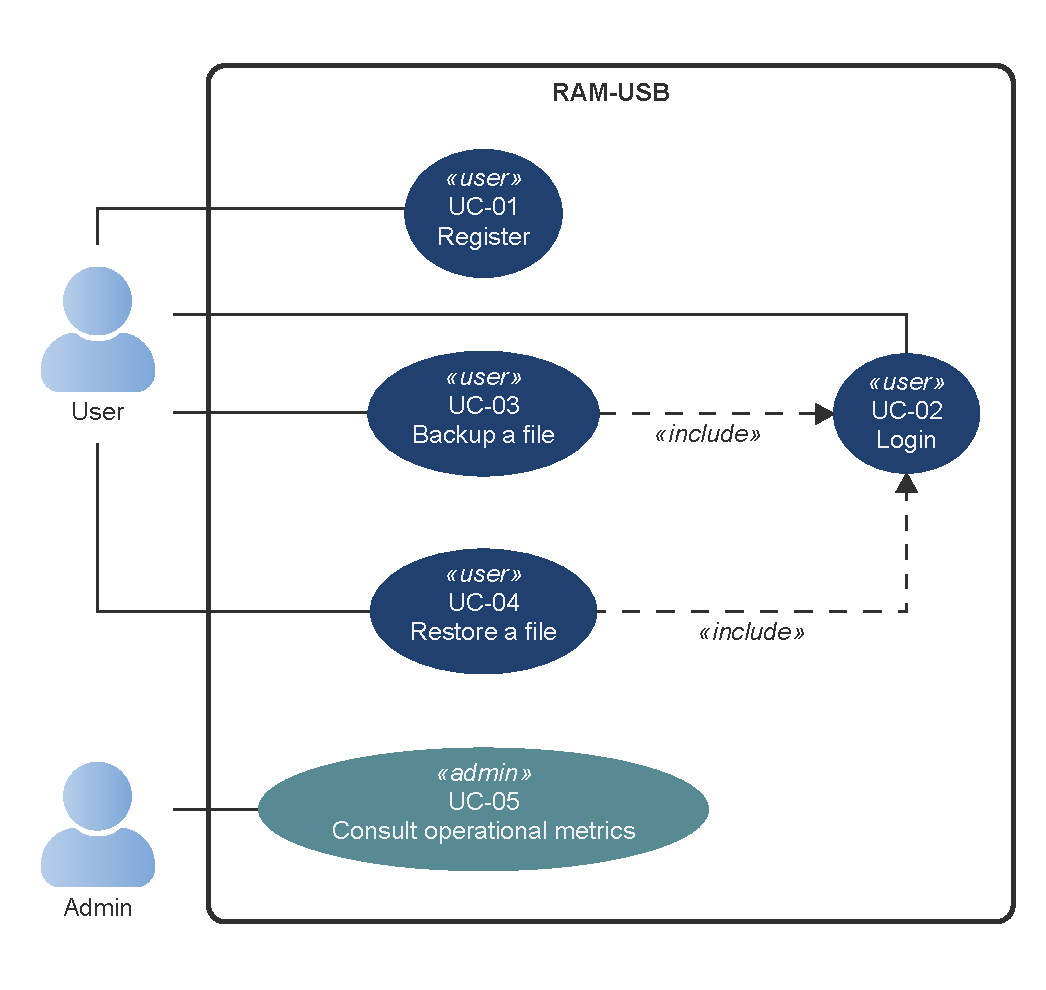
\includegraphics[width=0.5\textwidth]{figures/00-usecases-overview.pdf}
    \caption{Use case diagram of RAM-USB's main use cases.}
    \label{fig:usecases-overview}
\end{figure}

The following chapters describe how the architecture of the system realizes these use cases:
\autoref{chap:architettura} introduces the overall structure of the components and the security boundaries between
them, while Chapters 5--8 examine each functional domain in detail.
